\documentclass{article}
\usepackage[utf8]{inputenc}
\usepackage{graphicx}

\title{314-fun-problems}
\author{Matthew Chin}
\date{December 10, 2020}

\begin{document}

\maketitle

\section{Introduction}
\paragraph{}These are some of the responses to the MATH 314 fun problems. 

\section{2.3}

\paragraph{}By folding the overhead knot with the thin strip of paper, a perfect regular pentagon is formed because of the regular polygons that are made after the knot is formed. The perfect regular pentagon is formed by at minimum three isosceles trapezoids. If folding the rest of the strip of paper, more and more of these isosceles trapezoids will be formed in the shape of the regular pentagon. A regular pentagon has a total of 720 degrees with its five sides, which means that each angle is 144 degrees. Forming a knot with a strip of paper results in the formation of several trapezoids, mostly isosceles, with the exception of the ends which are trapezoids with two right angles which may be the ends of the strip of paper being used to make a knot around. Keep folding around the pentagon formed by the regular knot, and more and more trapezoids will form over a course of layers. 

\section{2.4}
\paragraph{}Any red marks seen on the square sheet of paper used are as means of showing where folds were made. These were not done with use of a ruler or with any other measuring device. 

\begin{figure}[h]
    \centering
    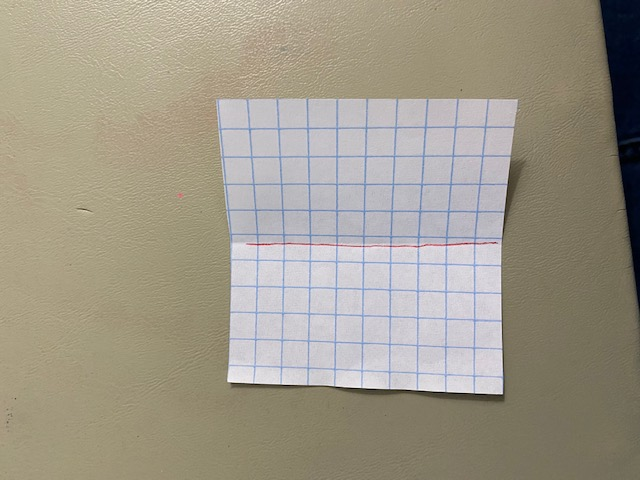
\includegraphics[width=3cm, height=3cm]{IMG_3174.jpg}
    \caption{First fold at the start.}
    \label{fig:my_label}
\end{figure}

Take a square sheet of paper or cut a sheet of paper that can be eyeballed as if it were a squared shape. Fold the paper in half, either horizontally or vertically. Having the paper faced with the longer side downward, take either the bottom left or the bottom right of that rectangle. Take one of the top ends of the rectangle and make a diagonal line. This means that if folding from the top left, the diagonal line goes to the bottom right vertex. If folding from the top right, the diagonal line goes to the bottom left vertex. A right scalene triangle will be formed, and although not aligned, there will exist another right scalene triangle. 

\begin{figure}[t]
    \centering
    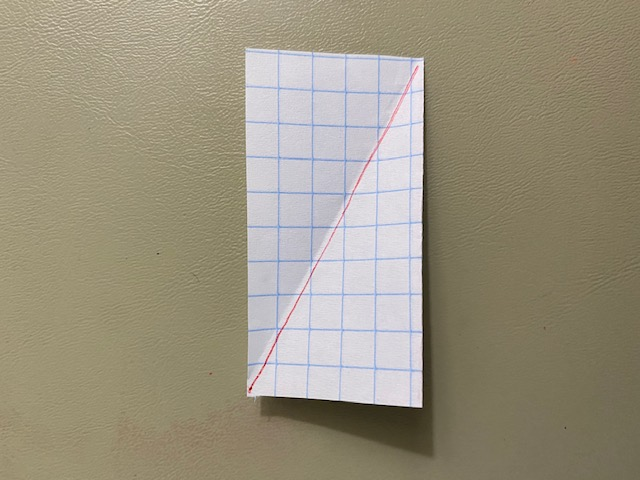
\includegraphics[height=3cm]{IMG_3175.jpg}
    \caption{Making a right scalene triangle. }
    \label{fig:my_label}
\end{figure}

Unfold all areas to return to the square sheet of paper. Lines are drawn to show where the folds have been made. It can be seen that a triangle is formed, and that all that needs to be done is to flip the outer right scalene triangles inward or behind the front face to create the equilateral triangle that is already seen. Do this to both of these right scalene triangles until no more of the hanging triangles can be seen when looking upfront. "Hiding" the triangles behind the front will be similar to folding formations for a basic paper airplane, as shown below in the subsequent images.

Flip the sheet of paper back to the front and it can be seen that there is an equilateral triangle. Rotate it several times and all three sides are to be of the same length. 

\begin{figure}[h]
    \centering
    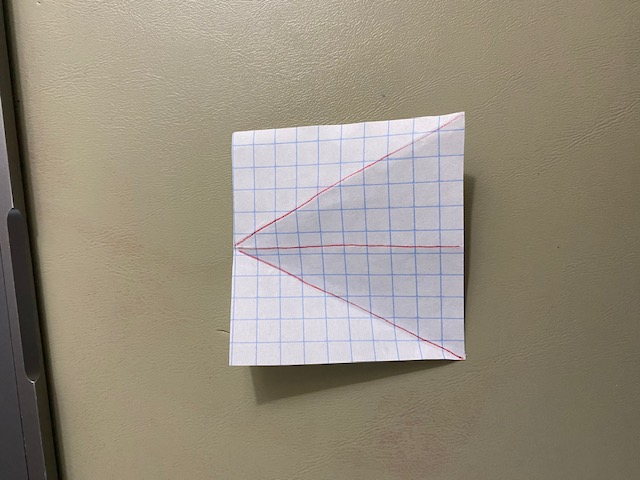
\includegraphics[width=3cm, height=3cm]{IMG_3176.jpg}
    \caption{All folds made to the sheet of paper. }
    \label{fig:my_label}
\end{figure}

\begin{figure}[h]
    \centering
    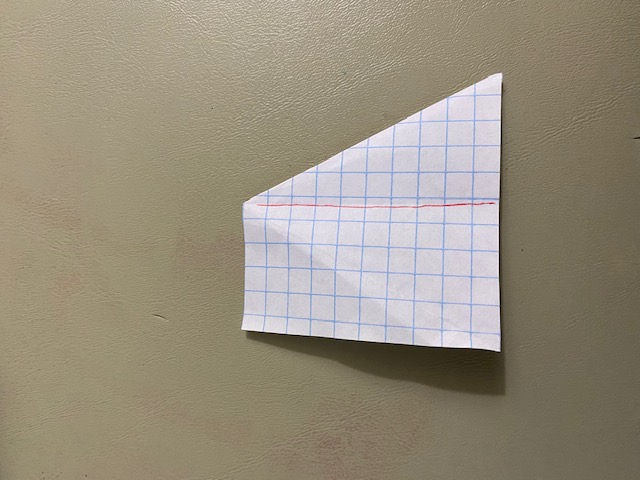
\includegraphics[width=3cm, height=3cm]{IMG_3177.jpg}
    \caption{Fold one of the outer triangles inward. }
    \label{fig:my_label}
\end{figure}

\begin{figure}[h]
    \centering
    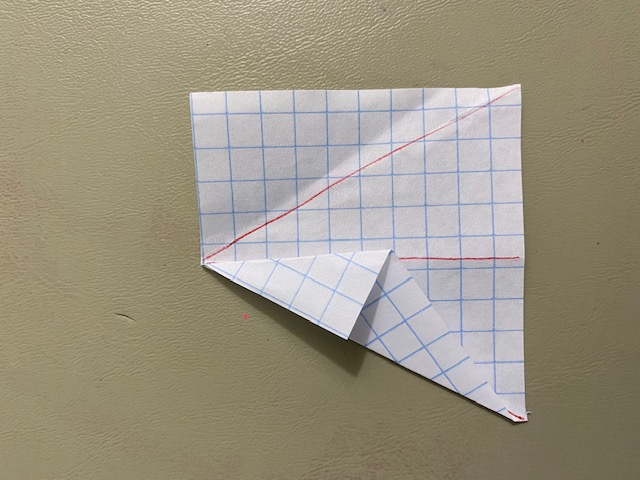
\includegraphics[width=3cm, height=3cm]{IMG_3178.jpg}
    \caption{Then fold the other outer triangle inward. }
    \label{fig:my_label}
\end{figure}

\begin{figure}[h]
    \centering
    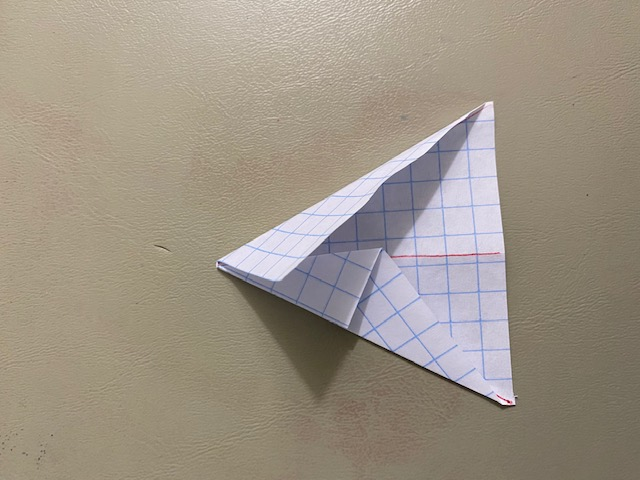
\includegraphics[width=3cm, height=3cm]{IMG_3179.jpg}
    \caption{Folding one of the triangle "flaps" inwards, behind the front of the triangle. }
    \label{fig:my_label}
\end{figure}

\begin{figure}[h]
    \centering
    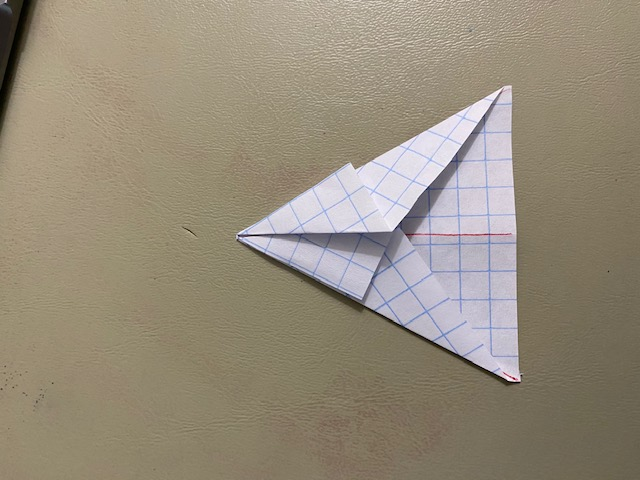
\includegraphics[width=3cm, height=3cm]{IMG_3180.jpg}
    \caption{The "flaps" folded inward behind the triangle front similar to making a paper plane. }
    \label{fig:my_label}
\end{figure}

\begin{figure}[h]
    \centering
    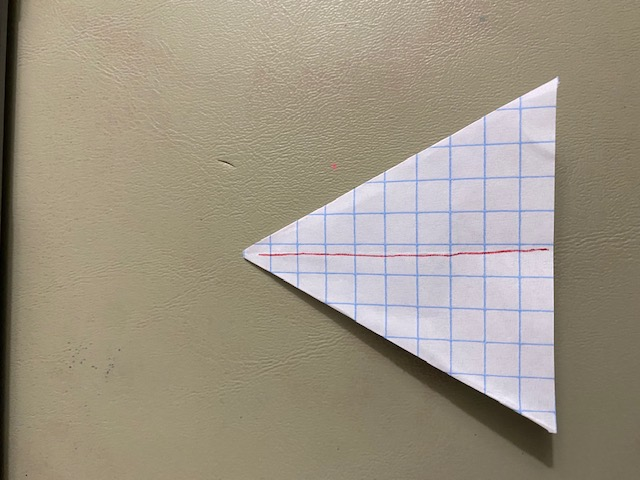
\includegraphics[width=3cm, height=3cm]{IMG_3185.jpg}
    \caption{Back to the front, the equilateral triangle can be seen.}
    \label{fig:my_label}
\end{figure}

\begin{figure}[h]
    \centering
    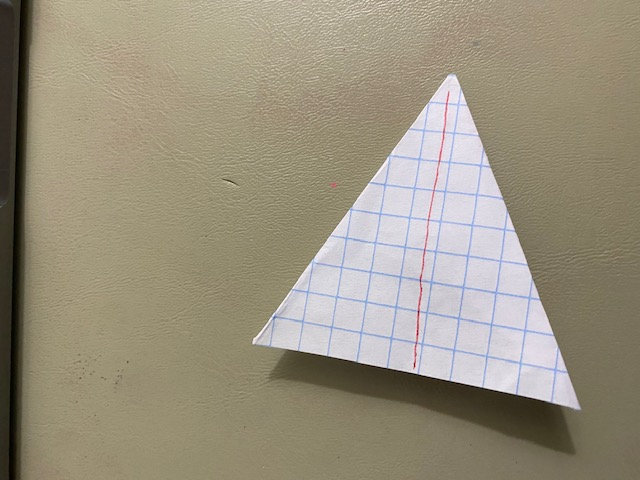
\includegraphics[width=4cm, height=4cm]{IMG_3186.jpg}
    \caption{Back to the front, the equilateral triangle can be seen.}
    \label{fig:my_label}
\end{figure}

\begin{figure}[h]
    \centering
    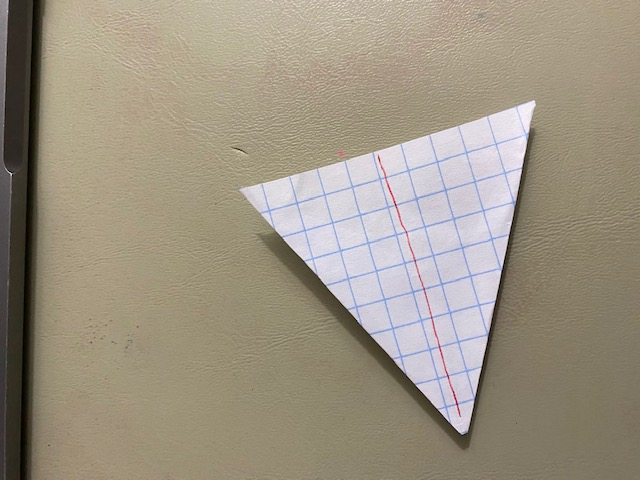
\includegraphics[width=4cm, height=4cm]{IMG_3187.jpg}
    \caption{Back to the front, the equilateral triangle can be seen.}
    \label{fig:my_label}
\end{figure}

\begin{figure}[h]
    \centering
    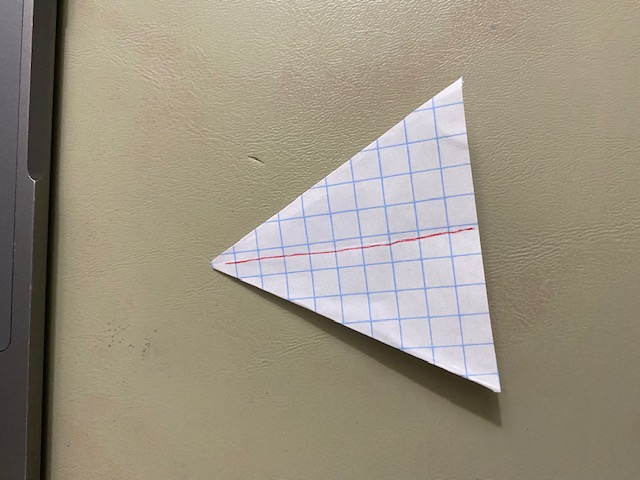
\includegraphics[width=4cm, height=4cm]{IMG_3188.jpg}
    \caption{Back to the front, the equilateral triangle can be seen.}
    \label{fig:my_label}
\end{figure}
\end{document}
